% Provenance (never printed): see sources/outline_sources.md (Year 1: optical
% mineralogy with the polarising microscope; Michel-Levy chart). Interference
% colours in figdata/bachelor-1/michel_levy.py from the CIE 1931 colour-matching
% functions and illuminant D65 (data/derived/bachelor-1-cie*.csv); exercise and
% problem values in the Book 3 scratch calculator calc/ch08.py.
\chapter{Minéralogie optique}\label{ch:b1:optical-mineralogy}

Entre \omterm{def:b1:field-lab-methods-1:microscope}{polariseurs croisés}, une \omterm{def:b1:field-lab-methods-1:thin-section}{lame mince} de gabbro s'illumine comme un vitrail.
De longues lattes grises et blanches, rayées comme un code-barres, traversent le
champ~; entre elles, des grains brillent en bleu, en jaune et en magenta~;
quelques-uns restent noirs quel que soit l'angle. Chacun de ces effets a une
cause que l'on peut calculer, et chacun dit quel \omterm{def:b1:rock-forming-minerals:mineral}{minéral} est là. Ce chapitre
explique comment la lumière traverse un cristal, pourquoi un \omterm{def:b1:rock-forming-minerals:mineral}{minéral} entre
\omterm{def:b1:field-lab-methods-1:microscope}{polariseurs croisés} est coloré, comment la couleur mesure une propriété du
\omterm{def:b1:rock-forming-minerals:mineral}{minéral}, et comment un pétrologue nomme les grains d'une \omterm{def:b1:field-lab-methods-1:thin-section}{lame mince} avec pour
seul instrument un microscope. Il se termine par une lame inconnue dont on
trouve les minéraux, et l'\omterm{def:b1:cross-sections:thickness}{épaisseur réelle}, d'après ce qu'elle montre.

\begin{recall}
Une \omterm{def:b1:field-lab-methods-1:thin-section}{lame mince} est une tranche de roche d'environ \qty{30}{\micro m} d'épaisseur
sur une lame de verre~; le \omterm{def:b1:field-lab-methods-1:microscope}{microscope polarisant} la regarde en \omterm{def:b1:field-lab-methods-1:microscope}{lumière polarisée
non analysée} (un seul polariseur) et entre \omterm{def:b1:field-lab-methods-1:microscope}{polariseurs croisés}
(\cref{ch:b1:field-lab-methods-1}). L'indice de réfraction $n$ d'un milieu est le
rapport de la vitesse de la lumière dans le vide à sa vitesse dans le milieu, et
la réfraction à une interface obéit à la loi de Snell--Descartes
$n_1\sin i_1 = n_2\sin i_2$ (physique, volume de première année). La lumière est
une onde transversale~; un polariseur ne laisse passer que la composante du champ
électrique le long de sa direction, de sorte qu'un analyseur faisant l'angle
$\alpha$ avec lui laisse passer la fraction $\cos^2\alpha$ de l'intensité (loi de
Malus, physique).
\end{recall}

\section{La lumière dans les cristaux}

Dans un verre, un liquide ou un cristal cubique, la lumière se propage à la même
vitesse dans toutes les directions et quelle que soit sa direction de vibration.
Dans la plupart des minéraux, il n'en est rien~: l'arrangement des atomes diffère
selon les directions, et la réponse des électrons au champ électrique de l'onde
aussi.

\begin{definition}[Minéraux isotropes et anisotropes]\label{def:b1:optical-mineralogy:anisotropic}
Un \omterm{def:b1:rock-forming-minerals:mineral}{minéral} est un \emph{minéral isotrope}\index{mineral isotrope@minéral isotrope} lorsque son indice de
réfraction est le même pour toute direction de propagation et de vibration de la
lumière~; les minéraux cubiques (\omterm{def:b1:rock-forming-minerals:groups}{grenat}, halite, spinelle) et les verres sont
isotropes. Il est un \emph{minéral anisotrope}\index{mineral anisotrope@minéral anisotrope}
lorsque son indice de réfraction dépend de la direction de vibration~; tous les
minéraux des autres systèmes cristallins sont anisotropes.
\end{definition}

Une lame taillée dans un cristal anisotrope ne laisse pas passer la lumière comme
une onde unique. On admet le résultat suivant de l'optique cristalline (physique,
volume de deuxième année)~: pour une direction de propagation donnée, une lame
d'un \omterm{def:b1:optical-mineralogy:anisotropic}{minéral anisotrope} transmet deux ondes qui vibrent selon deux directions
perpendiculaires fixées dans la lame, ses \emph{directions de vibration}, et se
propagent avec deux indices de réfraction différents $n_1$ et $n_2$. La lumière
qui vibre selon l'une de ces directions traverse la lame sans changer de
polarisation~; la lumière qui vibre selon toute autre direction est décomposée en
ses deux composantes selon elles. Les deux indices dépendent de la direction de
propagation, et il existe des directions particulières dans lesquelles ils sont
égaux.

\begin{definition}[Axe optique, minéraux uniaxes et biaxes]\label{def:b1:optical-mineralogy:optic-axis}
Un \emph{axe optique}\index{axe optique} d'un \omterm{def:b1:optical-mineralogy:anisotropic}{minéral anisotrope} est une direction de propagation le long de
laquelle la lumière se propage avec un seul indice de réfraction, quelle que soit
sa direction de vibration, comme dans un milieu isotrope. Un \omterm{def:b1:rock-forming-minerals:mineral}{minéral} est
\emph{uniaxe}\index{uniaxe} lorsqu'il a un axe optique (minéraux des systèmes
trigonal, quadratique et hexagonal, comme le quartz et la calcite) et
\emph{biaxe}\index{biaxe} lorsqu'il en a deux (minéraux orthorhombiques,
monocliniques et tricliniques, comme l'\omterm{def:b1:rock-forming-minerals:groups}{olivine}, les \omterm{def:b1:rock-forming-minerals:groups}{pyroxènes}, les \omterm{def:b1:rock-forming-minerals:groups}{amphiboles},
les \omterm{def:b1:rock-forming-minerals:groups}{micas} et les \omterm{def:b1:rock-forming-minerals:groups}{feldspaths}).
\end{definition}

La géométrie se résume par une surface, l'indicatrice~: un ellipsoïde dont le
rayon dans chaque direction est l'indice de réfraction pour la lumière vibrant
dans cette direction. La section de l'ellipsoïde perpendiculaire à la direction
de propagation est une ellipse dont les axes sont les deux directions de
vibration et dont les demi-axes sont $n_1$ et $n_2$. Pour un \omterm{def:b1:rock-forming-minerals:mineral}{minéral} \omterm{def:b1:optical-mineralogy:optic-axis}{uniaxe},
l'ellipsoïde est de révolution autour de l'\omterm{def:b1:optical-mineralogy:optic-axis}{axe optique}, avec deux indices
principaux $n_\omega$ et $n_\varepsilon$~: le quartz a $n_\omega = 1.544$ et
$n_\varepsilon = 1.553$, la calcite $1.658$ et $1.486$.
% ledger: hom:quartz-optics, hom:calcite-optics
Un \omterm{def:b1:rock-forming-minerals:mineral}{minéral} \omterm{def:b1:optical-mineralogy:optic-axis}{biaxe} a trois indices principaux $n_\alpha < n_\beta < n_\gamma$ et
deux sections circulaires, perpendiculaires à ses deux \omterm{def:b1:optical-mineralogy:optic-axis}{axes optiques}~: la
forstérite a $1.635$, $1.651$ et $1.670$.
% ledger: hom:forsterite-optics

\begin{definition}[Biréfringence (d'un minéral)]\label{def:b1:optical-mineralogy:birefringence}
La \emph{biréfringence}\index{birefringence (d'un mineral)@biréfringence (d'un minéral)} d'un \omterm{def:b1:rock-forming-minerals:mineral}{minéral} est la différence
$\delta = n_{\max} - n_{\min}$ entre son plus grand et son plus petit indice de
réfraction principal~: $n_\varepsilon - n_\omega$ en valeur absolue pour un
\omterm{def:b1:rock-forming-minerals:mineral}{minéral} \omterm{def:b1:optical-mineralogy:optic-axis}{uniaxe}, $n_\gamma - n_\alpha$ pour un \omterm{def:b1:rock-forming-minerals:mineral}{minéral} \omterm{def:b1:optical-mineralogy:optic-axis}{biaxe}. Dans un grain coupé
selon toute autre direction, la différence $|n_1 - n_2|$ est comprise entre 0
(une section perpendiculaire à un \omterm{def:b1:optical-mineralogy:optic-axis}{axe optique}) et $\delta$ (une section contenant
les directions de $n_{\max}$ et de $n_{\min}$).
\end{definition}

La \omterm{def:b1:optical-mineralogy:birefringence}{biréfringence} est une propriété du \omterm{def:b1:rock-forming-minerals:mineral}{minéral}, comme sa masse volumique~: quartz
\num{0.009}, calcite \num{0.172}, forstérite \num{0.035}, fayalite
\num{0.052}. Une \omterm{def:b1:field-lab-methods-1:thin-section}{lame mince} coupe les grains d'un \omterm{def:b1:rock-forming-minerals:mineral}{minéral} selon toutes les
orientations, de sorte que ses grains montrent toutes les valeurs de 0 à
$\delta$~; seule la plus haute est caractéristique.
% ledger: hom:quartz-optics, hom:calcite-optics, hom:forsterite-optics, hom:fayalite-optics

\section{Observations en lumière polarisée non analysée}

Avec le seul polariseur inférieur, le microscope montre la forme des grains, leur
couleur, leurs clivages et leur \omterm{def:b1:optical-mineralogy:relief}{relief}.

\begin{definition}[Pléochroïsme]\label{def:b1:optical-mineralogy:pleochroism}
Un \omterm{def:b1:rock-forming-minerals:mineral}{minéral} est \emph{pléochroïque}\index{pleochroisme@pléochroïsme} lorsque sa couleur, vue en \omterm{def:b1:field-lab-methods-1:microscope}{lumière polarisée
non analysée}, change quand la platine tourne~; le
\emph{pléochroïsme} est ce changement. Il tient à ce que l'absorption de la
lumière dépend de sa direction de vibration dans le cristal.
\end{definition}

La biotite est le cas d'école~: un grain coupé en travers de son clivage passe du
jaune-brun pâle au brun foncé en tournant, le plus foncé lorsque les traces de
clivage sont le long du polariseur. La hornblende passe du jaune au vert. La
plupart des autres silicates des roches (quartz, \omterm{def:b1:rock-forming-minerals:groups}{feldspaths}, \omterm{def:b1:rock-forming-minerals:groups}{olivine}, diopside,
muscovite) sont incolores en \omterm{def:b1:field-lab-methods-1:thin-section}{lame mince}, et leurs grains incolores se distinguent
par d'autres moyens.
% ledger: hom:biotite-optics, hom:hornblende-optics, hom:muscovite-optics, hom:diopside-optics, hom:forsterite-optics

\begin{definition}[Relief, liseré de Becke]\label{def:b1:optical-mineralogy:relief}
Le \emph{relief}\index{relief (optique)} d'un grain en \omterm{def:b1:field-lab-methods-1:thin-section}{lame mince} est la netteté avec laquelle son
contour, ses fissures et sa surface ressortent sur le milieu de montage~; il est
fort lorsque les indices de réfraction du grain et du milieu diffèrent beaucoup,
faible lorsqu'ils sont proches. Le \emph{liseré de Becke}\index{lisere de Becke@liseré de Becke}
est la fine ligne brillante qui borde un grain dont l'indice diffère de celui de
son environnement lorsque la mise au point du microscope est légèrement décalée.
\end{definition}

\begin{proposition}[Relief et indice de réfraction]\label{prop:b1:optical-mineralogy:relief}
Un rayon qui traverse sous l'incidence $i$ une frontière entre un milieu de
montage d'indice $n_m$ et un grain d'indice $n$ voisin de $n_m$ est dévié de
\[
  \varepsilon \approx \frac{|n - n_m|}{n_m}\,\tan i
\]
(en radians), au premier \omterm{def:b1:optical-mineralogy:interference-colour}{ordre} en $(n - n_m)/n_m$. Les déviations aux bords
inclinés d'un grain, et donc son \omterm{def:b1:optical-mineralogy:relief}{relief}, croissent proportionnellement à
$|n - n_m|$.
\end{proposition}

\begin{proof}
La loi de Snell--Descartes donne $n_m \sin i = n \sin r$. Écrivons
$n = n_m(1 + \eta)$ avec $\eta$ petit et $r = i - \varepsilon$ avec $\varepsilon$
petit. Alors
$\sin i = (1 + \eta)(\sin i - \varepsilon\cos i) + O(\eta^2, \varepsilon^2)$,
donc $\eta \sin i = \varepsilon\cos i$ au premier \omterm{def:b1:optical-mineralogy:interference-colour}{ordre}, c'est-à-dire
$\varepsilon = \eta\tan i$, avec $|\eta| = |n - n_m|/n_m$.
\end{proof}

Une \omterm{def:b1:field-lab-methods-1:thin-section}{lame mince} est montée dans une résine d'indice voisin de $1.54$.
% ledger: jaic:epoxy-ri
Le quartz ($1.544$--$1.553$) et les \omterm{def:b1:rock-forming-minerals:groups}{feldspaths} ($1.52$--$1.59$) y sont presque
invisibles~: \omterm{def:b1:optical-mineralogy:relief}{relief} faible, limites de grains difficiles à voir. L'\omterm{def:b1:rock-forming-minerals:groups}{olivine}
($1.64$--$1.88$), les \omterm{def:b1:rock-forming-minerals:groups}{pyroxènes} et les \omterm{def:b1:rock-forming-minerals:groups}{amphiboles} ressortent avec des bords
sombres et une surface d'aspect rugueux~: \omterm{def:b1:optical-mineralogy:relief}{relief} fort. Le \omterm{def:b1:rock-forming-minerals:groups}{grenat} ($1.83$) paraît
presque cerné de noir. La calcite, dont l'indice va de $1.486$ à $1.658$ avec la
direction de vibration, change de \omterm{def:b1:optical-mineralogy:relief}{relief} quand la platine tourne, un effet appelé
scintillement.
Le \omterm{def:b1:optical-mineralogy:relief}{relief} dit seulement de combien $n$ est éloigné de $n_m$, non de quel côté~; le
\omterm{def:b1:optical-mineralogy:relief}{liseré de Becke} dit le côté.
% ledger: hom:quartz-optics, hom:albite-optics, hom:anorthite-optics, hom:orthoclase-optics, hom:forsterite-optics, hom:fayalite-optics, hom:almandine-optics, hom:calcite-optics

\begin{method}[Le test du liseré de Becke]\label{met:b1:optical-mineralogy:becke}
Faire la mise au point sur le bord d'un grain en \omterm{def:b1:field-lab-methods-1:microscope}{lumière polarisée non analysée},
fermer un peu le diaphragme d'ouverture, et remonter légèrement la mise au point
(éloigner l'objectif de la lame). Le \omterm{def:b1:optical-mineralogy:relief}{liseré de Becke} brillant se déplace dans le
milieu d'indice de réfraction le plus élevé~: s'il se déplace dans le grain, le
grain a l'indice le plus élevé (\omterm{def:b1:optical-mineralogy:relief}{relief} positif)~; s'il en sort vers la résine ou
le grain voisin, le grain a l'indice le plus faible (\omterm{def:b1:optical-mineralogy:relief}{relief} négatif).
\end{method}

La méthode fonctionne parce qu'une limite de grain n'est jamais exactement
verticale~: à une limite inclinée, la lumière est réfractée vers le côté d'indice
le plus élevé, et au-delà de l'angle critique elle est totalement réfléchie de ce
côté, si bien que la lumière qui traverse la limite se concentre au-dessus du
milieu d'indice le plus élevé. Remonter la mise au point regarde un plan situé
au-dessus de la lame, où cette lumière concentrée se trouve à l'intérieur du
matériau d'indice le plus élevé.

\section{Entre polariseurs croisés}

Avec l'analyseur inséré, à angle droit du polariseur, un grain isotrope est noir
dans toutes les positions~: la lumière l'atteint en vibrant selon le polariseur et
le quitte en vibrant de la même façon, et l'analyseur l'arrête entièrement. Un
grain anisotrope est généralement brillant et coloré. La raison est la \omterm{def:b1:optical-mineralogy:retardation}{différence
de marche} entre ses deux ondes.

\begin{definition}[Différence de marche (dans une lame cristalline)]\label{def:b1:optical-mineralogy:retardation}
La \emph{différence de marche}\index{difference de marche (dans une lame cristalline)@différence de marche (dans une lame cristalline)} $\Delta$ d'une lame d'un \omterm{def:b1:optical-mineralogy:anisotropic}{minéral anisotrope} est la
différence entre les chemins optiques de ses deux ondes à la sortie de la lame,
l'onde la plus lente étant en retard sur la plus rapide.
\end{definition}

\begin{proposition}[Différence de marche et biréfringence]\label{prop:b1:optical-mineralogy:retardation}
Une lame d'épaisseur $d$ dont les deux ondes ont les indices $n_1 > n_2$ a la
\omterm{def:b1:optical-mineralogy:retardation}{différence de marche}
\[
  \Delta = d\,(n_1 - n_2),
\]
et ses deux ondes en sortent avec un déphasage $\varphi = 2\pi\Delta/\lambda$
pour une lumière de longueur d'onde $\lambda$ dans le vide. Dans une \omterm{def:b1:field-lab-methods-1:thin-section}{lame mince},
la plus grande \omterm{def:b1:optical-mineralogy:retardation}{différence de marche} que montrent les grains d'un même \omterm{def:b1:rock-forming-minerals:mineral}{minéral} est
$d\,\delta$.
\end{proposition}

\begin{proof}
Une onde qui traverse une épaisseur $d$ à la vitesse $c/n$ met le temps $nd/c$~;
son chemin optique, la distance que la lumière parcourrait dans le vide pendant ce
temps, est $nd$. Les deux ondes entrent ensemble~; à la sortie, la plus lente est
en retard de $n_1 d - n_2 d = d(n_1 - n_2)$, retard qui est la fraction
$\Delta/\lambda$ d'une période, c'est-à-dire un déphasage $2\pi\Delta/\lambda$.
La plus grande valeur de $n_1 - n_2$ parmi toutes les orientations est $\delta$
(\cref{def:b1:optical-mineralogy:birefringence}).
\end{proof}

Un grain de quartz de l'orientation la plus favorable dans une lame de
\qty{30}{\micro m} d'épaisseur a $\Delta = \qty{30000}{nm}\times0.009 =
\qty{270}{nm}$~; un grain de calcite $\qty{30000}{nm}\times0.172 = \qty{5160}{nm}$.

\begin{omfigure}
\begin{tikzpicture}[x=1cm, y=1cm, >={Stealth},
  sub/.style={align=center, font=\small, text width=4.2cm}]
% (a) the polariser
\begin{scope}
  \draw[gray!60] (-1.4,0) -- (1.4,0) (0,-1.4) -- (0,1.4);
  \node[gray, font=\scriptsize] at (1.55,-0.2) {E};
  \node[gray, font=\scriptsize] at (0.2,1.55) {N};
  \draw[very thick, omDef, <->] (-1.2,0) -- (1.2,0);
  \node[omDef, font=\scriptsize, above] at (0.75,0.05) {$E_0$};
  \node[sub] at (0,-2.1) {(a) après le polariseur~:\\ vibration est--ouest};
\end{scope}
% (b) inside the plate
\begin{scope}[shift={(5.0,0)}]
  \draw[gray!60] (-1.4,0) -- (1.4,0) (0,-1.4) -- (0,1.4);
  \draw[omThm, thick] (-1.35*0.866,-1.35*0.5) -- (1.35*0.866,1.35*0.5);
  \draw[omThm, thick] (1.35*0.5,-1.35*0.866) -- (-1.35*0.5,1.35*0.866);
  \node[omThm, font=\scriptsize] at (1.42,0.95) {1};
  \node[omThm, font=\scriptsize] at (-0.85,1.32) {2};
  \draw[very thick, omDef, ->] (0,0) -- (1.2,0);
  \draw[omProp, very thick, ->] (0,0) -- (1.2*0.866*0.866,1.2*0.866*0.5);
  \draw[omProp, very thick, ->] (0,0) -- (1.2*0.5*0.5,-1.2*0.5*0.866);
  \draw[densely dotted] (1.2,0) -- (1.2*0.866*0.866,1.2*0.866*0.5) (1.2,0) -- (1.2*0.5*0.5,-1.2*0.5*0.866);
  \draw (0.55,0) arc[start angle=0, end angle=30, radius=0.55];
  \node[font=\scriptsize] at (0.75,0.17) {$\theta$};
  \node[omProp, font=\scriptsize] at (0.45,1.0) {$E_0\cos\theta$};
  \node[omProp, font=\scriptsize, anchor=east] at (0.1,-0.85) {$E_0\sin\theta$};
  \node[sub] at (0,-2.1) {(b) dans la lame~: deux ondes selon\\ les directions de vibration 1 et 2};
\end{scope}
% (c) at the analyser
\begin{scope}[shift={(10.0,0)}]
  \draw[gray!60] (-1.4,0) -- (1.4,0);
  \draw[very thick, omMeth, <->] (0,-1.3) -- (0,1.3);
  \node[omMeth, font=\scriptsize, right] at (0.05,1.2) {analyseur};
  \draw[omProp, very thick, ->] (0,0) -- (1.2*0.866*0.866,1.2*0.866*0.5);
  \draw[omProp, very thick, ->] (0,0) -- (1.2*0.5*0.5,-1.2*0.5*0.866);
  \draw[densely dotted] (1.2*0.866*0.866,1.2*0.866*0.5) -- (0,1.2*0.866*0.5)
                        (1.2*0.5*0.5,-1.2*0.5*0.866) -- (0,-1.2*0.5*0.866);
  \draw[omMeth, very thick, ->] (0,0) -- (0,1.2*0.866*0.5);
  \draw[omMeth, very thick, ->] (0,0) -- (0,-1.2*0.5*0.866);
  \node[omMeth, font=\scriptsize, anchor=east] at (-0.08,0.52) {$+E_0\sin\theta\cos\theta$};
  \node[omMeth, font=\scriptsize, anchor=east] at (-0.08,-0.52) {$-E_0\sin\theta\cos\theta$};
  \node[sub] at (0,-2.1) {(c) à l'analyseur~: chaque onde\\ passe sa composante nord--sud};
\end{scope}
\end{tikzpicture}

{\small La lumière à travers une lame cristalline entre \omterm{def:b1:field-lab-methods-1:microscope}{polariseurs croisés}. Le
polariseur laisse passer la vibration est--ouest (a)~; la lame la sépare en deux
ondes selon ses directions de vibration, à $\theta$ et $\theta + \ang{90}$ du
polariseur (b)~; l'analyseur, nord--sud, laisse passer la composante nord--sud de
chacune (c). Les deux composantes ont des grandeurs égales et des signes
opposés~: sans le retard, elles s'annulent et la lame paraît sombre~; l'onde 2 est
en retard sur l'onde 1 du déphasage $\varphi = 2\pi\Delta/\lambda$, et la somme ne
s'annule plus.}
\end{omfigure}

\begin{theorem}[Intensité entre polariseurs croisés]\label{thm:b1:optical-mineralogy:intensity}
Une lame de \omterm{def:b1:optical-mineralogy:retardation}{différence de marche} $\Delta$ dont les directions de vibration font
l'angle $\theta$ avec le polariseur, entre \omterm{def:b1:field-lab-methods-1:microscope}{polariseurs croisés}, transmet à la
longueur d'onde $\lambda$ l'intensité
\[
  I = I_0\,\sin^2 2\theta\,\sin^2\frac{\pi\Delta}{\lambda},
\]
où $I_0$ est l'intensité qui sort du polariseur.
\end{theorem}

\begin{proof}
Prenons le polariseur selon $x$ et l'analyseur selon $y$, et écrivons le champ
sortant du polariseur comme la partie réelle de $E_0 e^{i\omega t}$ selon $x$,
avec $I_0 = E_0^2$ à une constante près. La direction de vibration 1 de la lame
est le vecteur unitaire $(\cos\theta, \sin\theta)$, la direction 2 est
$(-\sin\theta, \cos\theta)$. Le champ incident a pour composantes
$E_0\cos\theta$ selon 1 et
$-E_0\sin\theta$ selon 2. La lame laisse l'onde 1 inchangée, à une phase commune
près, et retarde l'onde 2 de $\varphi = 2\pi\Delta/\lambda$
(\cref{prop:b1:optical-mineralogy:retardation})~; en amplitudes complexes, les
ondes qui sortent de la lame sont $E_0\cos\theta$ selon 1 et
$-E_0\sin\theta\,e^{-i\varphi}$ selon 2. Leurs composantes selon $y$ sont
$E_0\cos\theta\sin\theta$ et $-E_0\sin\theta\cos\theta\,e^{-i\varphi}$~;
l'analyseur laisse passer leur somme,
\[
  A = E_0\sin\theta\cos\theta\,(1 - e^{-i\varphi}) .
\]
Comme $|1 - e^{-i\varphi}|^2 = 2 - 2\cos\varphi = 4\sin^2(\varphi/2)$ et
$\sin\theta\cos\theta = \frac12\sin2\theta$, l'intensité est
$|A|^2 = E_0^2\,\sin^2 2\theta\,\sin^2(\varphi/2)$, c'est-à-dire
$I = I_0\sin^2 2\theta\sin^2(\pi\Delta/\lambda)$. Si l'onde 1 est la plus lente,
$\varphi$ change de signe et $I$ est inchangé.
\end{proof}

Le théorème contient tout ce que montre le microscope entre \omterm{def:b1:field-lab-methods-1:microscope}{polariseurs croisés}.
Son premier facteur ne dépend que de l'orientation du grain sur la platine~; le
second, seulement de la \omterm{def:b1:optical-mineralogy:retardation}{différence de marche} du grain et de la couleur de la
lumière.

\begin{definition}[Position d'extinction, angle d'extinction]\label{def:b1:optical-mineralogy:extinction}
Un grain anisotrope entre \omterm{def:b1:field-lab-methods-1:microscope}{polariseurs croisés} est en \emph{position
d'extinction}\index{position d'extinction} lorsqu'il est sombre parce que ses directions de vibration sont
parallèles au polariseur et à l'analyseur. L'\emph{angle d'extinction}\index{angle d'extinction} d'un
grain est l'angle entre une direction visible dans le grain (une trace de
clivage, un allongement, un plan de \omterm{def:b1:optical-mineralogy:twin}{macle}) et la position d'extinction la plus
proche, lu sur la platine graduée.
\end{definition}

Le facteur $\sin^2 2\theta$ s'annule pour $\theta = 0$, \ang{90}, \ang{180} et
\ang{270}~: un grain devient sombre quatre fois par tour complet de la platine, et
est le plus brillant à mi-chemin, à \ang{45} de l'extinction (figure ci-dessous).
Un grain avec
$\Delta = 0$ --- un \omterm{def:b1:optical-mineralogy:anisotropic}{minéral isotrope}, ou une section perpendiculaire à un \omterm{def:b1:optical-mineralogy:optic-axis}{axe
optique} --- reste sombre en permanence. L'\omterm{def:b1:optical-mineralogy:extinction}{angle d'extinction} dépend de la symétrie
du cristal~: un \omterm{def:b1:rock-forming-minerals:mineral}{minéral} dont les directions de vibration sont liées à ses
clivages, comme les minéraux orthorhombiques, s'éteint parallèlement à eux
(extinction droite)~; un \omterm{def:b1:rock-forming-minerals:mineral}{minéral} monoclinique ou triclinique ne le fait
généralement pas (extinction oblique). Le plus grand \omterm{def:b1:optical-mineralogy:extinction}{angle d'extinction} entre les
traces de clivage et la direction de vibration lente est d'environ \ang{38} dans
le diopside et de \ang{15}--\ang{19} dans la hornblende, dans des sections
parallèles à $(010)$~: l'une des façons de distinguer un \omterm{def:b1:rock-forming-minerals:groups}{pyroxène} d'une \omterm{def:b1:rock-forming-minerals:groups}{amphibole}
en \omterm{def:b1:field-lab-methods-1:thin-section}{lame mince}.
% ledger: hom:diopside-optics, hom:hornblende-optics

\begin{omfigure}
\begin{tikzpicture}
\begin{axis}[width=0.8\linewidth, height=5cm, xmin=0, xmax=360, ymin=0, ymax=1.08,
  xtick={0,45,90,...,360}, ytick={0,0.5,1},
  tick label style={font=\scriptsize}, label style={font=\small},
  xlabel={angle de la platine $\theta$ depuis une position d'extinction (\si{\degree})},
  ylabel={$I/I_0$}, legend style={font=\scriptsize, at={(0.5,1.03)}, anchor=south, legend columns=3,
  draw=none}, legend cell align=left]
\addplot[omThm, thick] table[x=theta, y=I270] {figdata/out/bachelor-1-michel_levy-rotation.dat};
\addplot[omDef, thick, densely dashed] table[x=theta, y=I100] {figdata/out/bachelor-1-michel_levy-rotation.dat};
\addplot[omMeth, thick, densely dotted] table[x=theta, y=I540] {figdata/out/bachelor-1-michel_levy-rotation.dat};
\legend{$\Delta = \qty{270}{nm}$, $\Delta = \qty{100}{nm}$, $\Delta = \qty{540}{nm}$}
\end{axis}
\end{tikzpicture}

{\small L'intensité laissée passer par un grain quand la platine tourne, à la
longueur d'onde \qty{550}{nm}, pour trois \omterm{def:b1:optical-mineralogy:retardation}{différences de marche}
(\cref{thm:b1:optical-mineralogy:intensity}). Quatre extinctions par tour, quatre
maxima à \ang{45} d'elles~; la \omterm{def:b1:optical-mineralogy:retardation}{différence de marche} fixe la hauteur des maxima,
qui est presque nulle lorsque $\Delta$ est proche d'un nombre entier de longueurs
d'onde.}
\end{omfigure}

\subsection{Teintes de polarisation}

En lumière blanche, le second facteur $\sin^2(\pi\Delta/\lambda)$ agit comme un
filtre qui dépend de la longueur d'onde. Un grain avec $\Delta = \qty{270}{nm}$
laisse passer presque tout le vert et le jaune ($\lambda$ voisin de
$2\Delta = 540$\,nm, où le facteur vaut 1) et un peu moins du violet et du rouge~:
il paraît blanc. Un grain avec $\Delta = \qty{550}{nm}$ supprime le jaune-vert
($\lambda = \Delta$) et laisse passer le rouge et le bleu~: il paraît magenta.
Quand $\Delta$ croît, les longueurs d'onde supprimées se déplacent sur le spectre
et de nouvelles apparaissent, et la couleur parcourt une suite fixe.

\begin{definition}[Teinte de polarisation, ordre, abaque de Michel-Lévy]\label{def:b1:optical-mineralogy:interference-colour}
La \emph{teinte de polarisation}\index{teinte de polarisation} d'un grain anisotrope est sa couleur entre \omterm{def:b1:field-lab-methods-1:microscope}{polariseurs
croisés} en lumière blanche, à \ang{45} de l'extinction~; elle ne dépend que de sa
\omterm{def:b1:optical-mineralogy:retardation}{différence de marche} $\Delta$. Les couleurs se répètent par bandes d'environ
\qty{550}{nm} de \omterm{def:b1:optical-mineralogy:retardation}{différence de marche}, chacune se terminant par une teinte
rouge-violet~; chaque bande est un \emph{ordre}\index{ordre (d'une teinte de polarisation)}
(premier, deuxième, troisième\dots). L'\emph{abaque de Michel-Lévy}\index{abaque de Michel-Levy@abaque de Michel-Lévy} montre les teintes de polarisation en
fonction de la \omterm{def:b1:optical-mineralogy:retardation}{différence de marche}, avec les droites $\Delta = d\,\delta$ qui
relient l'épaisseur d'une section, la \omterm{def:b1:optical-mineralogy:birefringence}{biréfringence} d'un \omterm{def:b1:rock-forming-minerals:mineral}{minéral} et sa couleur.
\end{definition}

\begin{omfigure}
\begin{tikzpicture}
\begin{axis}[width=0.84\linewidth, height=7.2cm, view={0}{90}, xmin=0, xmax=1800, ymin=0, ymax=50,
  xtick={0,200,...,1800}, ytick={0,10,...,50}, axis on top, clip=false,
  tick label style={font=\scriptsize}, label style={font=\small},
  xlabel={différence de marche $\Delta$ (nm)}, ylabel={épaisseur $d$ (\si{\micro m})},
  unbounded coords=jump]
\addplot3[surf, shader=flat corner, mesh/cols=361, mesh/color input=explicit mathparse,
  point meta={symbolic={\thisrow{r},\thisrow{g},\thisrow{b}}}]
  table[x=delta, y=d, z expr=0] {figdata/out/bachelor-1-michel_levy-chart.dat};
\addplot3[black, thin] table[x=x, y=y, z expr=0] {figdata/out/bachelor-1-michel_levy-segments.dat};
\addplot3[white, very thick, densely dashed] coordinates {(0,30,0) (1800,30,0)};
\node[font=\tiny, anchor=south west, rotate=60] at (axis cs:250,50.3,0) {orthose 0.005};
\node[font=\tiny, anchor=south west, rotate=60] at (axis cs:450,50.3,0) {quartz 0.009};
\node[font=\tiny, anchor=south west, rotate=60] at (axis cs:600,50.3,0) {plagioclase 0.012};
\node[font=\tiny, anchor=south west, rotate=60] at (axis cs:1000,50.3,0) {hornblende 0.020};
\node[font=\tiny, anchor=south west, rotate=60] at (axis cs:1500,50.3,0) {diopside 0.030};
\node[font=\tiny, anchor=south west, rotate=60] at (axis cs:1750,50.3,0) {forstérite 0.035};
\node[font=\tiny, anchor=west] at (axis cs:1810,45,0) {muscovite 0.040};
\node[font=\tiny, anchor=west] at (axis cs:1810,34.6,0) {fayalite 0.052};
\node[font=\tiny, anchor=west] at (axis cs:1810,10.5,0) {calcite 0.172};
\node[font=\tiny, anchor=west] at (axis cs:1810,30,0) {\qty{30}{\micro m}};
\node[font=\scriptsize, anchor=north] at (axis cs:270,-7,0) {premier ordre};
\node[font=\scriptsize, anchor=north] at (axis cs:808,-7,0) {deuxième ordre};
\node[font=\scriptsize, anchor=north] at (axis cs:1340,-7,0) {troisième ordre};
\end{axis}
\end{tikzpicture}

{\small Un \omterm{def:b1:optical-mineralogy:interference-colour}{abaque de Michel-Lévy} calculé à partir des premiers principes~: pour
chaque \omterm{def:b1:optical-mineralogy:retardation}{différence de marche}, la couleur de la lumière blanche (illuminant standard
CIE D65) à travers des \omterm{def:b1:field-lab-methods-1:microscope}{polariseurs croisés} et une lame à \ang{45} de l'extinction,
d'après les fonctions colorimétriques CIE 1931 (données \textcopyright{} CIE,
CC BY-SA 4.0) et la transformation sRGB, normalisée à la lumière laissée passer
par des polariseurs parallèles. Les droites noires donnent $\Delta = d\,\delta$
pour la \omterm{def:b1:optical-mineralogy:birefringence}{biréfringence} de chaque \omterm{def:b1:rock-forming-minerals:mineral}{minéral}~; la droite en tirets est l'épaisseur
standard de \qty{30}{\micro m}. Les teintes rouge-violet qui terminent les \omterm{def:b1:optical-mineralogy:interference-colour}{ordres}
tombent à 542, 1074 et \qty{1605}{nm} dans ce calcul.}
% ledger: data:b3-cie1931, data:b3-cie-d65, w3c:srgb, hom:orthoclase-optics, hom:quartz-optics, hom:albite-optics, hom:anorthite-optics, hom:hornblende-optics, hom:diopside-optics, hom:forsterite-optics, hom:muscovite-optics, hom:fayalite-optics, hom:calcite-optics
\end{omfigure}

L'abaque est calculé exactement comme le dit le théorème. Pour chaque \omterm{def:b1:optical-mineralogy:retardation}{différence
de marche}, chaque longueur d'onde de la lumière est pondérée par
$\sin^2(\pi\Delta/\lambda)$~; le spectre transmis est ensuite converti en une
couleur telle que l'œil la voit, par les fonctions colorimétriques standard de la
colorimétrie, puis en rouge, vert et bleu d'un écran ou d'une imprimante par la
transformation sRGB. Trois traits méritent d'être remarqués. Le premier \omterm{def:b1:optical-mineralogy:interference-colour}{ordre}
commence noir, passe par le gris et le blanc (le seul blanc de l'abaque est près
de \qty{270}{nm}, où le spectre est presque entièrement transmis), puis le jaune,
l'orange et le rouge. Les deuxième et troisième \omterm{def:b1:optical-mineralogy:interference-colour}{ordres} sont les plus brillants,
avec des bleus, verts, jaunes et magentas vifs. Au-delà du quatrième \omterm{def:b1:optical-mineralogy:interference-colour}{ordre}, les
couleurs s'estompent~: lorsque $\Delta$ vaut de nombreuses longueurs d'onde, le
filtre $\sin^2(\pi\Delta/\lambda)$ oscille plusieurs fois sur le spectre visible,
laisse passer chaque couleur tour à tour et, en moyenne, la moitié de la lumière~:
le grain paraît gris pâle rosé ou verdâtre, le blanc d'\omterm{def:b1:optical-mineralogy:interference-colour}{ordre} élevé de la calcite.

Lire l'abaque est le cœur de la minéralogie optique. Dans une section d'épaisseur
connue, la plus haute couleur que montre un \omterm{def:b1:rock-forming-minerals:mineral}{minéral} donne sa \omterm{def:b1:optical-mineralogy:birefringence}{biréfringence}~:
suivre l'épaisseur jusqu'à la couleur, puis la droite passant par ce point
jusqu'à sa \omterm{def:b1:optical-mineralogy:birefringence}{biréfringence}. Inversement, un \omterm{def:b1:rock-forming-minerals:mineral}{minéral} de \omterm{def:b1:optical-mineralogy:birefringence}{biréfringence} connue donne
l'épaisseur~: dans une bonne section de \qty{30}{\micro m}, le quartz ne montre
jamais plus qu'un blanc de premier \omterm{def:b1:optical-mineralogy:interference-colour}{ordre} ou le jaune le plus pâle, et une section
où le quartz montre du jaune ou de l'orange est trop épaisse.

\begin{history}[Auguste Michel-Lévy]
% ledger: annales:michel-levy, annales:michel-levy-director, commons:michel-levy
\begin{minipage}[t]{0.76\linewidth}\vspace{0pt}
Auguste Michel-Lévy (1844--1911), qui devint directeur du Service de la carte
géologique de France, fut l'un des premiers à identifier systématiquement les
minéraux des roches au \omterm{def:b1:field-lab-methods-1:microscope}{microscope polarisant}. Avant lui, les couleurs des minéraux
entre \omterm{def:b1:field-lab-methods-1:microscope}{polariseurs croisés} étaient employées de façon empirique~; il montra que ce
qui compte est la \omterm{def:b1:optical-mineralogy:birefringence}{biréfringence} maximale de chaque \omterm{def:b1:rock-forming-minerals:mineral}{minéral}, que l'on peut mesurer
en comparant les couleurs de ses grains à un coin de quartz dont la \omterm{def:b1:optical-mineralogy:retardation}{différence de
marche} croît régulièrement sur sa longueur. Avec son élève Alfred Lacroix, il
publia en 1888 \emph{Les minéraux des roches}, un manuel des propriétés optiques
des minéraux des roches. L'abaque qui porte son nom, des couleurs en fonction de
la \omterm{def:b1:optical-mineralogy:retardation}{différence de marche} avec des droites d'égale \omterm{def:b1:optical-mineralogy:birefringence}{biréfringence}, est toujours la
façon de lire les \omterm{def:b1:optical-mineralogy:interference-colour}{teintes de polarisation}.
\end{minipage}\hfill
\begin{minipage}[t]{0.2\linewidth}\vspace{0pt}
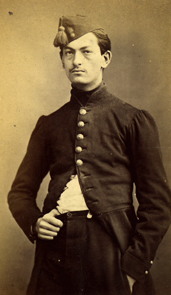
\includegraphics[width=\linewidth]{images/book3/b1-michel-levy.jpg}

{\scriptsize Michel-Lévy étudiant, vers 1862. Domaine public.}
\end{minipage}
\end{history}

Deux ondes qui sortent d'un grain peuvent recevoir une \omterm{def:b1:optical-mineralogy:retardation}{différence de marche}
supplémentaire connue grâce à une lame auxiliaire insérée au-dessus de la section
à \ang{45} des polariseurs. La plus courante est taillée pour montrer le rouge du
premier \omterm{def:b1:optical-mineralogy:interference-colour}{ordre} (lame de teinte sensible), une \omterm{def:b1:optical-mineralogy:retardation}{différence de marche} d'environ
\qty{540}{nm}. Si la direction de vibration lente du grain est parallèle à la
direction lente de la lame, les retards s'ajoutent et la couleur du grain monte
d'environ un \omterm{def:b1:optical-mineralogy:interference-colour}{ordre}~; si elle est parallèle à la direction rapide, ils se
retranchent et la couleur descend. Un grain gris de premier \omterm{def:b1:optical-mineralogy:interference-colour}{ordre} de \qty{100}{nm}
devient bleu de deuxième \omterm{def:b1:optical-mineralogy:interference-colour}{ordre} (\qty{640}{nm}) dans une orientation et orange de
premier \omterm{def:b1:optical-mineralogy:interference-colour}{ordre} (\qty{440}{nm}) dans l'autre~; le test montre laquelle des deux
directions de vibration du grain est la lente, propriété utilisée pour identifier
les minéraux allongés.

\section{Identifier les minéraux en lame mince}

\begin{definition}[Macle, macle polysynthétique]\label{def:b1:optical-mineralogy:twin}
Une \emph{macle}\index{macle} est une association de deux cristaux ou plus du même
\omterm{def:b1:rock-forming-minerals:mineral}{minéral} dont les réseaux sont reliés par une symétrie que le cristal n'a pas
lui-même, comme une réflexion par rapport à un plan (le plan de macle). Une
\emph{macle polysynthétique}\index{macle polysynthetique@macle polysynthétique} est une macle répétée sur des plans parallèles, qui
divise un cristal en minces lamelles parallèles dont les orientations alternent.
\end{definition}

Entre \omterm{def:b1:field-lab-methods-1:microscope}{polariseurs croisés}, les lamelles d'une \omterm{def:b1:optical-mineralogy:twin}{macle polysynthétique} s'éteignent
alternativement~: la moitié d'entre elles sont sombres lorsque l'autre moitié sont
brillantes, et le cristal paraît rayé. Le \omterm{def:b1:rock-forming-minerals:groups}{plagioclase} montre presque toujours ces
rayures, qui le distinguent aussitôt du quartz et du \omterm{def:b1:rock-forming-minerals:groups}{feldspath alcalin}~; son autre
caractère, un \omterm{def:b1:optical-mineralogy:relief}{relief} faible et des couleurs allant du gris au blanc de premier
\omterm{def:b1:optical-mineralogy:interference-colour}{ordre}, il le partage avec eux. Les \omterm{def:b1:optical-mineralogy:extinction}{angles d'extinction} des deux familles de
lamelles, mesurés de part et d'autre du plan de \omterm{def:b1:optical-mineralogy:twin}{macle}, dépendent de la
composition du \omterm{def:b1:rock-forming-minerals:groups}{plagioclase}, et des abaques de ces angles donnent sa teneur en
anorthite.

\begin{method}[Identifier un minéral en lame mince]\label{met:b1:optical-mineralogy:identify}
\begin{enumerate}
  \item En \omterm{def:b1:field-lab-methods-1:microscope}{lumière polarisée non analysée}~: noter si le grain est opaque~; sa
        couleur et son \omterm{def:b1:optical-mineralogy:pleochroism}{pléochroïsme} (tourner la platine)~; son \omterm{def:b1:optical-mineralogy:relief}{relief}, et de quel
        côté de $1.54$ se situe son indice (\omterm{def:b1:optical-mineralogy:relief}{liseré de Becke})~; sa forme et ses
        clivages, et l'angle entre deux clivages.
  \item Entre \omterm{def:b1:field-lab-methods-1:microscope}{polariseurs croisés}~: vérifier s'il reste sombre (isotrope, ou
        section perpendiculaire à un \omterm{def:b1:optical-mineralogy:optic-axis}{axe optique})~; parmi les grains d'un même
        \omterm{def:b1:rock-forming-minerals:mineral}{minéral}, trouver la plus haute \omterm{def:b1:optical-mineralogy:interference-colour}{teinte de polarisation} et lire la
        \omterm{def:b1:optical-mineralogy:birefringence}{biréfringence} sur l'\omterm{def:b1:optical-mineralogy:interference-colour}{abaque de Michel-Lévy} pour l'épaisseur de la
        section.
  \item Mesurer l'\omterm{def:b1:optical-mineralogy:extinction}{angle d'extinction} sur les grains montrant un clivage ou un
        allongement~; chercher les \omterm{def:b1:optical-mineralogy:twin}{macles} (rayures polysynthétiques, \omterm{def:b1:optical-mineralogy:twin}{macles}
        simples).
  \item Comparer avec un tableau de propriétés optiques
        (\cref{tab:b1:optical-mineralogy:key}) et avec les minéraux que la roche
        peut contenir (\cref{ch:b1:rock-forming-minerals}).
\end{enumerate}
\end{method}

\begin{table}[htbp]
\centering\footnotesize
\setlength{\tabcolsep}{3pt}
% ledger: hom:quartz-optics, hom:orthoclase-optics, hom:albite-optics, hom:anorthite-optics, hom:muscovite-optics, hom:biotite-optics, hom:hornblende-optics, hom:diopside-optics, hom:forsterite-optics, hom:fayalite-optics, hom:almandine-optics, hom:calcite-optics, hom:magnetite-optics
\begin{tabular}{@{}>{\raggedright\arraybackslash}p{2.0cm}>{\raggedright\arraybackslash}p{2.6cm}>{\raggedright\arraybackslash}p{2.3cm}>{\raggedright\arraybackslash}p{1.8cm}>{\raggedright\arraybackslash}p{3.0cm}>{\raggedright\arraybackslash}p{3.8cm}@{}}
\hline
\omterm{def:b1:rock-forming-minerals:mineral}{minéral} & couleur (LPNA) & indices & \omterm{def:b1:optical-mineralogy:birefringence}{biréfringence} & plus haute teinte à \qty{30}{\micro m} & autres caractères \\
\hline
quartz & incolore & 1.544--1.553 & 0.009 & blanc du premier \omterm{def:b1:optical-mineralogy:interference-colour}{ordre} & pas de clivage~; pas de \omterm{def:b1:optical-mineralogy:twin}{macles} visibles~; \omterm{def:b1:optical-mineralogy:optic-axis}{uniaxe} \\
orthose & incolore, souvent trouble & 1.518--1.525 & 0.005 & gris du premier \omterm{def:b1:optical-mineralogy:interference-colour}{ordre} & \omterm{def:b1:optical-mineralogy:relief}{relief} négatif~; \omterm{def:b1:optical-mineralogy:twin}{macles} simples \\
\omterm{def:b1:rock-forming-minerals:groups}{plagioclase} & incolore & 1.526--1.590 & 0.008--0.013 & blanc à jaune pâle du premier \omterm{def:b1:optical-mineralogy:interference-colour}{ordre} & \omterm{def:b1:optical-mineralogy:twin}{macle polysynthétique} \\
muscovite & incolore & 1.552--1.618 & 0.035--0.042 & teintes vives du deuxième au troisième \omterm{def:b1:optical-mineralogy:interference-colour}{ordre} & un clivage parfait~; extinction droite \\
biotite & brune, verte & 1.565--1.696 & 0.04--0.07 & masquée par sa propre couleur & fort \omterm{def:b1:optical-mineralogy:pleochroism}{pléochroïsme}~; un clivage parfait \\
hornblende & verte, brune & 1.675--1.695 & 0.020 & bleu du deuxième \omterm{def:b1:optical-mineralogy:interference-colour}{ordre} & \omterm{def:b1:optical-mineralogy:pleochroism}{pléochroïque}~; clivages à \ang{56}/\ang{124}~; extinction \ang{15}--\ang{19} \\
diopside & incolore & 1.664--1.694 & 0.030 & jaune du deuxième \omterm{def:b1:optical-mineralogy:interference-colour}{ordre} & clivages à environ \ang{87}/\ang{93}~; extinction d'environ \ang{38} \\
\omterm{def:b1:rock-forming-minerals:groups}{olivine} & incolore (Mg) à jaune pâle (Fe) & 1.635--1.879 & 0.035--0.052 & fin du deuxième \omterm{def:b1:optical-mineralogy:interference-colour}{ordre} au troisième \omterm{def:b1:optical-mineralogy:interference-colour}{ordre} & \omterm{def:b1:optical-mineralogy:relief}{relief} fort~; fissures irrégulières, pas de bon clivage \\
\omterm{def:b1:rock-forming-minerals:groups}{grenat} & incolore à rose pâle & 1.830 (almandin) & isotrope & noir & \omterm{def:b1:optical-mineralogy:relief}{relief} très fort~; contours à six ou huit côtés \\
calcite & incolore & 1.486--1.658 & 0.172 & blanc d'\omterm{def:b1:optical-mineralogy:interference-colour}{ordre} élevé & le \omterm{def:b1:optical-mineralogy:relief}{relief} change à la rotation~; clivage rhomboédrique \\
magnétite & opaque & --- & --- & --- & noire dans les deux modes d'éclairage \\
\hline
\end{tabular}
\caption{Propriétés optiques des minéraux courants des roches en \omterm{def:b1:field-lab-methods-1:thin-section}{lame mince}.
LPNA~: \omterm{def:b1:field-lab-methods-1:microscope}{lumière polarisée non analysée}. La plus haute teinte se lit sur l'\omterm{def:b1:optical-mineralogy:interference-colour}{abaque
de Michel-Lévy} à $\Delta = \qty{30000}{nm}\times\delta$.}
\label{tab:b1:optical-mineralogy:key}
\end{table}

\begin{omfigure}
\setlength{\tabcolsep}{2pt}
\begin{tabular}{cc}
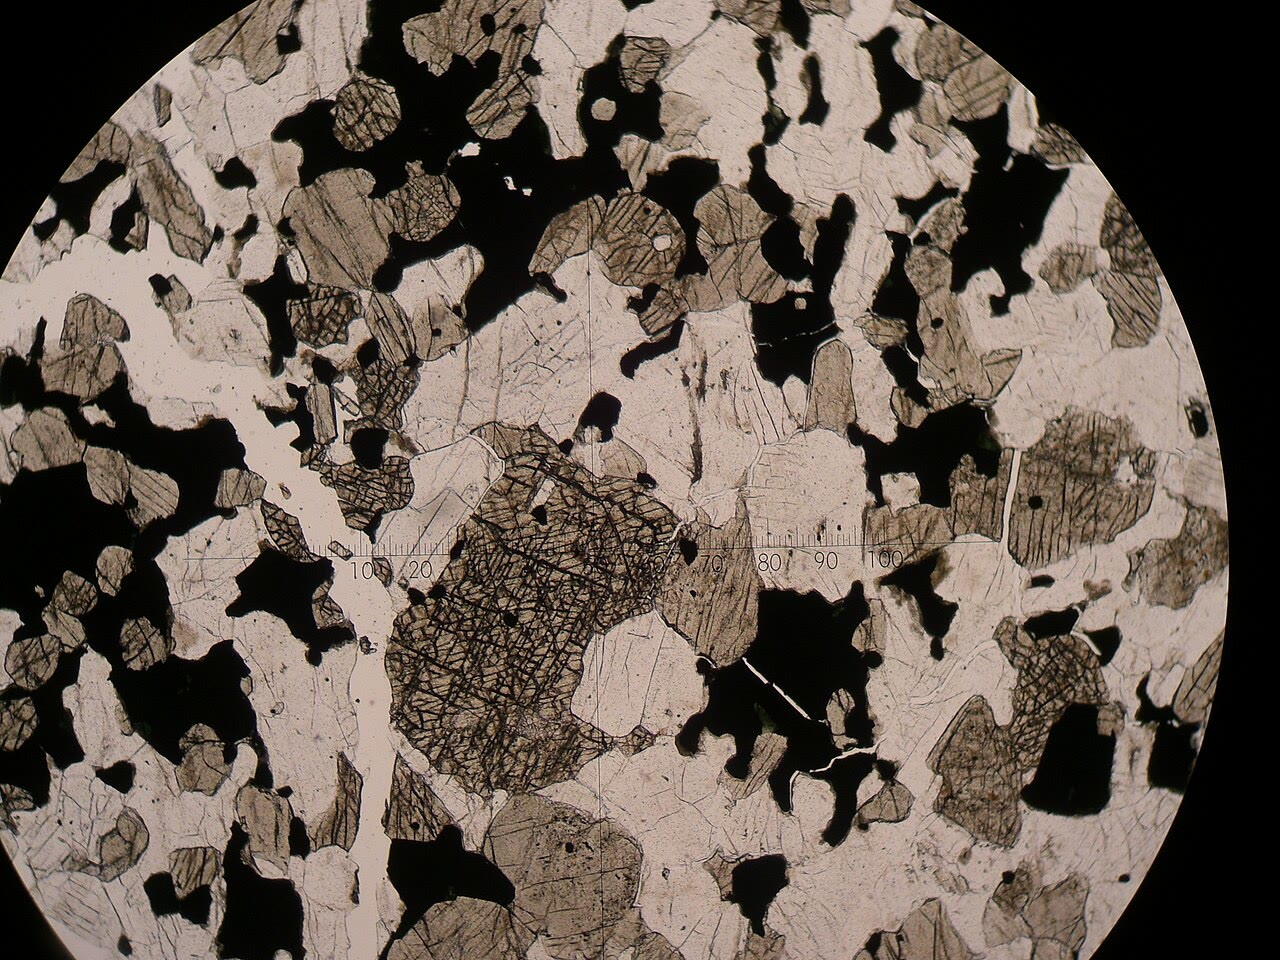
\includegraphics[width=0.485\linewidth]{images/book3/b1-gabbro-ppl.jpg} &
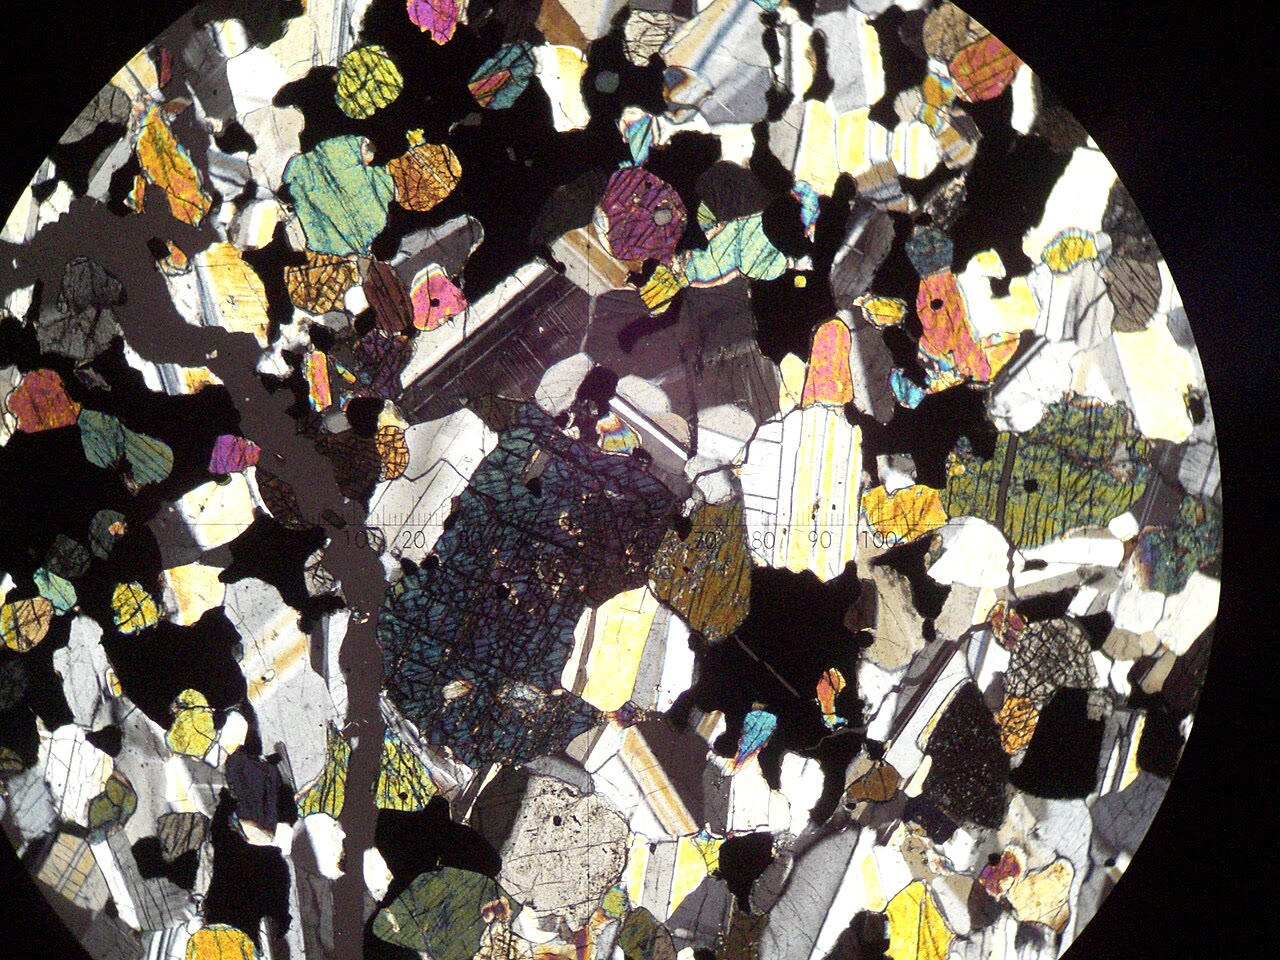
\includegraphics[width=0.485\linewidth]{images/book3/b1-gabbro-xpl.jpg} \\
{\small (a) \omterm{def:b1:field-lab-methods-1:microscope}{lumière polarisée non analysée}} & {\small (b) \omterm{def:b1:field-lab-methods-1:microscope}{polariseurs croisés}} \\
\end{tabular}
% ledger: commons:gabbro-ppl, commons:gabbro-xpl

\medskip
{\small Le même champ d'un gabbro en \omterm{def:b1:field-lab-methods-1:thin-section}{lame mince}. En \omterm{def:b1:field-lab-methods-1:microscope}{lumière polarisée non
analysée} (a), le \omterm{def:b1:rock-forming-minerals:groups}{plagioclase} est incolore à \omterm{def:b1:optical-mineralogy:relief}{relief} faible, les grains de \omterm{def:b1:rock-forming-minerals:groups}{pyroxène}
et d'\omterm{def:b1:rock-forming-minerals:groups}{olivine} sont gris-brun pâle à \omterm{def:b1:optical-mineralogy:relief}{relief} fort et fissures denses, et le minerai
opaque est noir~; l'échelle est un micromètre oculaire. Entre \omterm{def:b1:field-lab-methods-1:microscope}{polariseurs croisés}
(b), les lattes de \omterm{def:b1:rock-forming-minerals:groups}{plagioclase} sont rayées par la \omterm{def:b1:optical-mineralogy:twin}{macle polysynthétique}, les
grains de \omterm{def:b1:rock-forming-minerals:groups}{pyroxène} et d'\omterm{def:b1:rock-forming-minerals:groups}{olivine} brillent dans les teintes du deuxième \omterm{def:b1:optical-mineralogy:interference-colour}{ordre}, et
le minerai reste noir. Photographies Chmee2, CC BY-SA 3.0 (Wikimedia Commons).}
\end{omfigure}

\begin{inthelab}[Une séance au microscope]
\begin{minipage}[t]{0.55\linewidth}\vspace{0pt}
Une pétrologue qui décrit une nouvelle \omterm{def:b1:field-lab-methods-1:thin-section}{lame mince} la parcourt d'abord à faible
grossissement, pour voir la texture et les minéraux principaux, puis grain par
grain. Pour chaque \omterm{def:b1:rock-forming-minerals:mineral}{minéral}, elle consigne les observations de la méthode
ci-dessus, estime sa proportion dans le champ, et note comment les grains se
touchent~: lesquels ont cristallisé en premier, lesquels remplissent les espaces
laissés, lesquels en remplacent d'autres. Les mesures optiques se font avec la
platine graduée en degrés et une lame auxiliaire~; les compositions, lorsqu'elles
comptent, sont mesurées plus tard à la microsonde sur la même lame. Un
laboratoire d'enseignement fonctionne de la même façon, un microscope par
étudiant et, à côté, une boîte de lames de référence de minéraux connus.
\end{minipage}\hfill
\begin{minipage}[t]{0.42\linewidth}\vspace{0pt}
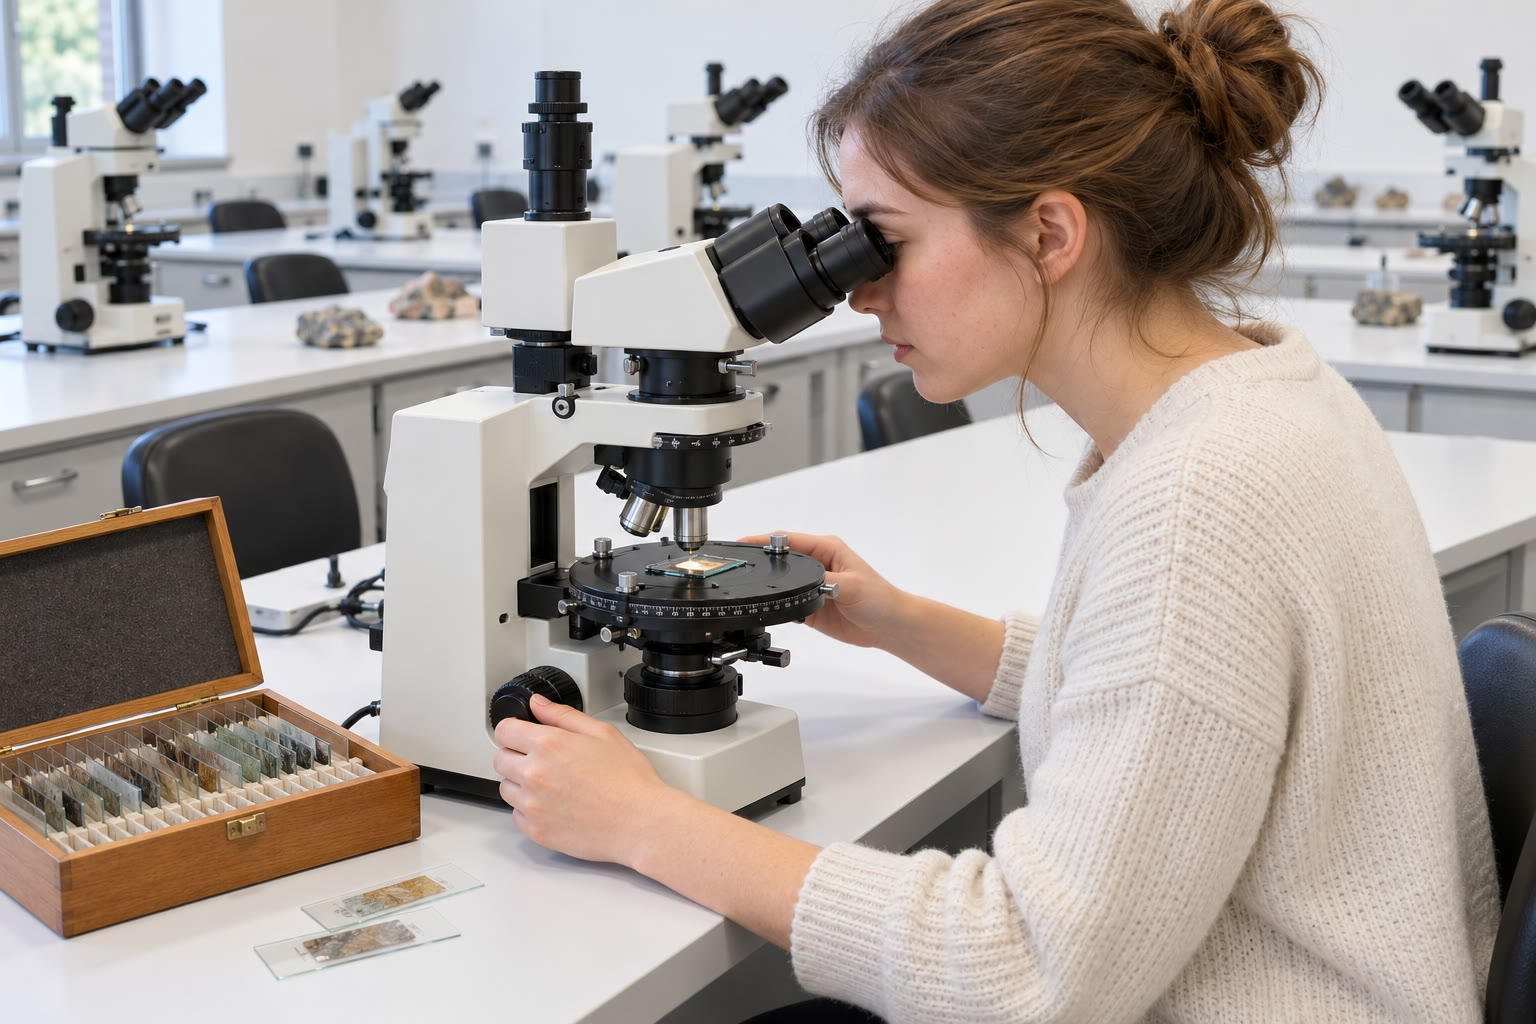
\includegraphics[width=\linewidth]{images/book3/ai/b1-microscope-student.jpg}

{\scriptsize Un étudiant à un \omterm{def:b1:field-lab-methods-1:microscope}{microscope polarisant} dans un laboratoire
d'enseignement (illustration générée par IA).}
\end{minipage}
\end{inthelab}

\section{Exercices}

\begin{exercise}[$\star$]\label{exo:b1:optical-mineralogy:1}
Calculer la plus grande \omterm{def:b1:optical-mineralogy:retardation}{différence de marche} du quartz ($\delta = 0.009$) et de
la calcite ($\delta = 0.172$) dans une section de \qty{30}{\micro m} d'épaisseur.
À l'aide de l'\omterm{def:b1:optical-mineralogy:interference-colour}{abaque de Michel-Lévy}, décrire la couleur de chacun.
% ledger: hom:quartz-optics, hom:calcite-optics
\end{exercise}

\begin{exercise}[$\star$]\label{exo:b1:optical-mineralogy:2}
Un grain est tourné sur la platine entre \omterm{def:b1:field-lab-methods-1:microscope}{polariseurs croisés}. Calculer $I/I_0$,
en fraction de son maximum, pour $\theta = 0$, \ang{22.5}, \ang{45}, \ang{67.5} et
\ang{90} depuis une \omterm{def:b1:optical-mineralogy:extinction}{position d'extinction}.
\end{exercise}

\begin{exercise}[$\star$]\label{exo:b1:optical-mineralogy:3}
Expliquer pourquoi un \omterm{def:b1:rock-forming-minerals:groups}{grenat} reste noir entre \omterm{def:b1:field-lab-methods-1:microscope}{polariseurs croisés} quelle que soit
la position de la platine, et pourquoi un grain de quartz peut faire de même.
Comment les distinguer en \omterm{def:b1:field-lab-methods-1:microscope}{lumière polarisée non analysée}~?
\end{exercise}

\begin{exercise}[$\star$]\label{exo:b1:optical-mineralogy:4}
Classer par \omterm{def:b1:optical-mineralogy:relief}{relief}, dans un milieu d'indice $1.54$, l'orthose ($n$ voisin de
$1.52$), le quartz ($1.55$), la forstérite ($1.65$) et l'almandin ($1.83$). Lequel
a un \omterm{def:b1:optical-mineralogy:relief}{relief} négatif~? Dans quelle direction son \omterm{def:b1:optical-mineralogy:relief}{liseré de Becke} se déplace-t-il
quand la mise au point est remontée~?
% ledger: hom:orthoclase-optics, hom:quartz-optics, hom:forsterite-optics, hom:almandine-optics
\end{exercise}

\begin{exercise}[$\star\star$]\label{exo:b1:optical-mineralogy:5}
Dans une section de \qty{30}{\micro m}, les grains d'un \omterm{def:b1:rock-forming-minerals:mineral}{minéral} vert \omterm{def:b1:optical-mineralogy:pleochroism}{pléochroïque}
à deux clivages à \ang{56} et \ang{124} montrent au plus un bleu du deuxième
\omterm{def:b1:optical-mineralogy:interference-colour}{ordre}, lu sur l'abaque comme $\Delta = \qty{650}{nm}$. Calculer sa \omterm{def:b1:optical-mineralogy:birefringence}{biréfringence}
et nommer le \omterm{def:b1:rock-forming-minerals:mineral}{minéral} à l'aide du \cref{tab:b1:optical-mineralogy:key}.
\end{exercise}

\begin{exercise}[$\star\star$]\label{exo:b1:optical-mineralogy:6}
À l'aide de la \cref{prop:b1:optical-mineralogy:relief} avec $n_m = 1.54$ et
$i = \ang{30}$, calculer la déviation au bord d'un grain de quartz
($n = 1.553$) et d'un grain de forstérite ($n = 1.651$), en degrés, et le
rapport des deux. Vérifier la seconde avec la loi de Snell--Descartes exacte.
\end{exercise}

\begin{exercise}[$\star\star$]\label{exo:b1:optical-mineralogy:7}
Une lame de teinte sensible rouge du premier \omterm{def:b1:optical-mineralogy:interference-colour}{ordre} a $\Delta = \qty{540}{nm}$. Un
grain de quartz de $\Delta = \qty{270}{nm}$ est placé à \ang{45} avec la lame
insérée. Quelles sont les deux \omterm{def:b1:optical-mineralogy:retardation}{différences de marche} totales possibles, et les
couleurs qu'elles donnent sur l'abaque~? Quelle orientation rend parallèles les
deux directions lentes~?
\end{exercise}

\begin{exercise}[$\star\star$]\label{exo:b1:optical-mineralogy:8}
À son bord aminci, un grain de fayalite ($\delta = 0.052$) passe de
\qty{30}{\micro m} à zéro. Combien de teintes rouge-violet, qui terminent les
\omterm{def:b1:optical-mineralogy:interference-colour}{ordres} à 542, 1074 et \qty{1605}{nm}, apparaissent comme franges colorées entre
le bord et la partie d'épaisseur pleine du grain~?
% ledger: hom:fayalite-optics
\end{exercise}

\begin{exercise}[$\star\star$]\label{exo:b1:optical-mineralogy:9}
Sur plusieurs grains allongés à un bon clivage, un géologue mesure des \omterm{def:b1:optical-mineralogy:extinction}{angles
d'extinction} de \ang{0}, \ang{21}, \ang{36} et \ang{37} entre la trace du clivage
et la direction de vibration lente. Pourquoi les valeurs diffèrent-elles~? Le
\omterm{def:b1:rock-forming-minerals:mineral}{minéral} est-il plus probablement du diopside ou de la hornblende~?
% ledger: hom:diopside-optics, hom:hornblende-optics
\end{exercise}

\begin{exercise}[$\star\star\star$]\label{exo:b1:optical-mineralogy:10}
Refaire la démonstration du \cref{thm:b1:optical-mineralogy:intensity} avec
l'analyseur parallèle au polariseur, et montrer que
$I_\parallel = I_0\bigl(1 - \sin^2 2\theta\sin^2(\pi\Delta/\lambda)\bigr)$.
Quelle couleur un grain de $\Delta = \qty{550}{nm}$ montre-t-il à \ang{45}
entre polariseurs parallèles~?
\end{exercise}

\begin{exercise}[$\star\star\star$]\label{exo:b1:optical-mineralogy:11}
Pour un grain de calcite avec $\Delta = \qty{5000}{nm}$, le facteur
$\sin^2(\pi\Delta/\lambda)$ s'annule chaque fois que $\Delta/\lambda$ est un
entier. (a) Combien de fois s'annule-t-il entre \num{400} et
\qty{700}{nm}~? (b) Montrer qu'au voisinage de $\lambda = \qty{550}{nm}$ deux
zéros successifs sont distants d'environ $\lambda^2/\Delta$, et le calculer. (c)
Expliquer pourquoi le grain paraît presque blanc.
\end{exercise}

\begin{exercise}[$\star\star\star$]\label{exo:b1:optical-mineralogy:12}
Montrer que, en moyenne sur un tour complet de la platine, un grain entre
\omterm{def:b1:field-lab-methods-1:microscope}{polariseurs croisés} laisse passer $\frac12 I_0\sin^2(\pi\Delta/\lambda)$. Une
géologue estime les \omterm{def:b1:optical-mineralogy:birefringence}{biréfringences} à partir de la plus haute teinte de chaque
\omterm{def:b1:rock-forming-minerals:mineral}{minéral}, en supposant \qty{30}{\micro m}, dans une section qui est en fait de
\qty{25}{\micro m} d'épaisseur. De quel facteur toutes ses valeurs sont-elles
fausses, et dans quel sens~?
\end{exercise}

\section{Problème~: Identifier les minéraux d'une lame mince inconnue}

\begin{problem}[{Problème du week-end --- observer le relief, le pléochroïsme et
les teintes de polarisation, mesurer l'épaisseur d'une section avec du quartz, et
nommer ses minéraux}]
\label{pb:b1:optical-mineralogy:1}
% values: calc/ch08.py; optical data: ledger hom:*-optics
% ledger: hom:quartz-optics, hom:diopside-optics, hom:forsterite-optics, hom:albite-optics, hom:anorthite-optics, hom:hornblende-optics, hom:biotite-optics
Une \omterm{def:b1:field-lab-methods-1:thin-section}{lame mince} d'une roche magmatique inconnue, montée dans une résine d'indice
$1.540$, est dite avoir \qty{30}{\micro m} d'épaisseur. Elle contient cinq
minéraux, notés de A à E. Utiliser le tableau des propriétés optiques du
chapitre, l'\omterm{def:b1:optical-mineralogy:interference-colour}{abaque de Michel-Lévy} et les valeurs suivantes~: quartz
$n_\omega = 1.544$, $n_\varepsilon = 1.553$~; diopside $n_\alpha = 1.664$,
$n_\beta = 1.672$, $n_\gamma = 1.694$.

\medskip
\noindent\textbf{Partie I --- Lumière polarisée non analysée.}
\begin{enumerate}
  \item Le \omterm{def:b1:rock-forming-minerals:mineral}{minéral} A est incolore, avec des limites de grains difficiles à voir.
        Le \omterm{def:b1:rock-forming-minerals:mineral}{minéral} B est incolore, avec de forts bords sombres et deux clivages
        se coupant à environ \ang{87}. Lequel a le \omterm{def:b1:optical-mineralogy:relief}{relief} le plus fort~?
  \item Pour A, pris comme du quartz, et B, pris comme du diopside, calculer
        $|n - n_m|$ en utilisant la moyenne des indices principaux de chacun.
  \item À l'aide de la \cref{prop:b1:optical-mineralogy:relief}, calculer le
        rapport des déviations à leurs bords pour la même inclinaison de la
        limite.
  \item Quand on remonte la mise au point, le \omterm{def:b1:optical-mineralogy:relief}{liseré de Becke} de B se déplace
        dans le grain. Que montre-t-il~?
  \item Le \omterm{def:b1:rock-forming-minerals:mineral}{minéral} C passe du jaune pâle au brun foncé quand la platine tourne,
        le plus foncé lorsque son unique clivage est le long du polariseur.
        Nommer la propriété et le \omterm{def:b1:rock-forming-minerals:mineral}{minéral}.
  \item Le \omterm{def:b1:rock-forming-minerals:mineral}{minéral} D est incolore, à faible \omterm{def:b1:optical-mineralogy:relief}{relief}, en longues lattes~; E est vert
        à jaune et \omterm{def:b1:optical-mineralogy:pleochroism}{pléochroïque}, avec deux clivages à \ang{124}. Que suggère
        l'angle pour E~?
\end{enumerate}

\medskip
\noindent\textbf{Partie II --- L'épaisseur de la section.}
\begin{enumerate}[resume]
  \item Quelle est la plus grande \omterm{def:b1:optical-mineralogy:retardation}{différence de marche} du quartz dans une section
        d'exactement \qty{30}{\micro m}~? Quelle couleur est-ce~?
  \item Pourquoi faut-il chercher la plus grande \omterm{def:b1:optical-mineralogy:retardation}{différence de marche} parmi de
        nombreux grains de A, plutôt que la mesurer sur l'un d'eux~?
  \item La plus haute teinte que montrent les grains de A est un jaune pâle du
        premier \omterm{def:b1:optical-mineralogy:interference-colour}{ordre}~; un comparateur à coin de quartz en donne la \omterm{def:b1:optical-mineralogy:retardation}{différence de
        marche}, \qty{342}{nm}. Calculer l'\omterm{def:b1:cross-sections:thickness}{épaisseur réelle} de la section.
  \item De combien pour cent la section est-elle plus épaisse qu'elle ne
        devrait~?
  \item À $\lambda = \qty{550}{nm}$ et à \ang{45} de l'extinction, calculer
        $I/I_0$ pour ce grain de quartz, et pour le même grain dans une section
        de \qty{30}{\micro m}.
  \item Calculer l'intervalle des \omterm{def:b1:optical-mineralogy:retardation}{différences de marche} de D, pris comme
        \omterm{def:b1:rock-forming-minerals:groups}{plagioclase} ($\delta = 0.008$ à $0.013$), dans cette section, et dire si
        ses couleurs restent dans le premier \omterm{def:b1:optical-mineralogy:interference-colour}{ordre}.
\end{enumerate}

\medskip
\noindent\textbf{Partie III --- La biréfringence de B.}
\begin{enumerate}[resume]
  \item La plus haute teinte de B est un bleu lu comme $\Delta = \qty{1140}{nm}$.
        De quel \omterm{def:b1:optical-mineralogy:interference-colour}{ordre} est-elle~?
  \item Calculer la \omterm{def:b1:optical-mineralogy:birefringence}{biréfringence} de B avec l'épaisseur trouvée à la question 9.
  \item Quelle \omterm{def:b1:optical-mineralogy:birefringence}{biréfringence} aurait-on trouvée en supposant \qty{30}{\micro m}~?
        Quel \omterm{def:b1:rock-forming-minerals:mineral}{minéral} incolore à \omterm{def:b1:optical-mineralogy:relief}{relief} fort cela aurait-il suggéré, et pourquoi
        est-il déplacé dans une roche contenant du quartz (considérer
        \ce{Mg2SiO4 + SiO2 -> 2 MgSiO3})~?
  \item Comparer le résultat de la question 14 au tableau, avec le \omterm{def:b1:optical-mineralogy:relief}{relief} et les
        clivages de B, et conclure.
  \item Quelle couleur B montrerait-il au plus dans une section correcte de
        \qty{30}{\micro m}~?
  \item La section est amincie jusqu'à \qty{30}{\micro m}. De combien faut-il
        l'amincir, et quelle est alors la plus haute teinte du quartz~?
\end{enumerate}

\medskip
\noindent\textbf{Partie IV --- Extinction et macles.}
\begin{enumerate}[resume]
  \item Les lattes de D sont divisées en bandes parallèles qui s'éteignent
        alternativement. Nommer ce caractère et le \omterm{def:b1:rock-forming-minerals:mineral}{minéral}.
  \item Les bandes d'une latte s'éteignent à \ang{27} et \ang{28} de part et
        d'autre du plan de \omterm{def:b1:optical-mineralogy:twin}{macle}. Que donnent de tels angles, mesurés sur de
        nombreuses lattes, une fois comparés à des abaques publiés~?
  \item Le plus grand \omterm{def:b1:optical-mineralogy:extinction}{angle d'extinction} entre les clivages de E et sa direction
        lente est de \ang{17}. Nommer E.
  \item Calculer la plus grande \omterm{def:b1:optical-mineralogy:retardation}{différence de marche} de E dans cette section et la
        couleur qu'elle montre.
  \item Un grain de B reste sombre pendant une rotation complète. Expliquer
        comment il peut être le même \omterm{def:b1:rock-forming-minerals:mineral}{minéral} que les grains brillants de B.
  \item Lister les minéraux A à E, et dire quelle sorte de roche ils forment.
  \item Quelle est l'\omterm{def:b1:cross-sections:thickness}{épaisseur réelle} de la section, en micromètres~?
\end{enumerate}
\end{problem}
